\documentclass[border=5pt,tikz]{standalone}
\usepackage{amsmath} % for \dfrac
\usepackage{physics}
\usepackage{tikz,pgfplots}
\usepackage[siunitx]{circuitikz} %[symbols]
\usepackage[outline]{contour} % glow around text
\usetikzlibrary{arrows,arrows.meta}
\usetikzlibrary{decorations.markings}
\usetikzlibrary{hobby}
\tikzset{>=latex} % for LaTeX arrow head
\usepackage{xcolor}
\colorlet{Icol}{blue!50!black}
\colorlet{Ccol}{orange!90!black}
\colorlet{Rcol}{green!50!black}
\colorlet{loopcol}{red!90!black!25}
\colorlet{pluscol}{red!60!black}
\colorlet{minuscol}{blue!60!black}
\newcommand\EMF{\mathcal{E}} %\varepsilon}
\contourlength{1.5pt}

\ctikzset{capacitors/width=0.4}
\tikzstyle{EMF}=[battery1,l=$\EMF$,invert]
\tikzstyle{internal R}=[R,color=Rcol,Rcol,l=$r$,/tikz/circuitikz/bipoles/length=30pt]
\tikzstyle{loop}=[->,red!90!black!25]
\tikzstyle{loop label}=[loopcol,fill=white,scale=0.8,inner sep=1]
\tikzstyle{thick R}=[R,color=Rcol,thick,Rcol,l=$R$]
\tikzstyle{thick C}=[C,thick,color=Ccol,Ccol]
\tikzstyle{myswitch}=[closing switch,line width=0.3] %-{Latex[length=3]},

\begin{document}


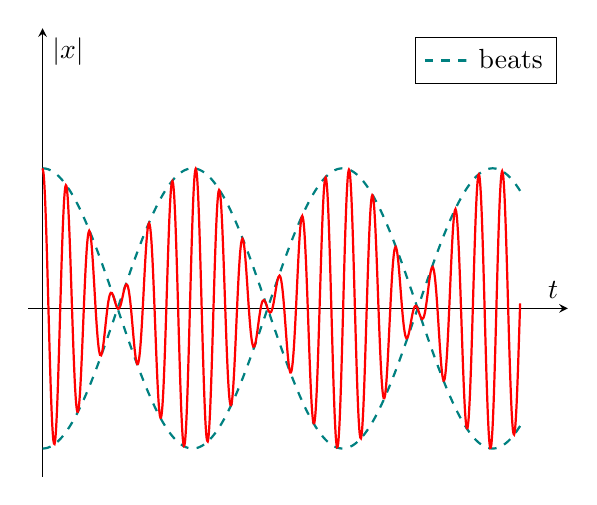
\begin{tikzpicture}
  \begin{axis} [axis lines=center,
    xlabel=$t$,
    ylabel=$|x|$,
    ticks=none,
    ymin = -1.2,
    ymax = 2,
    xmin = -0.3,
    xmax = 11.0]
    \addplot [domain=0:10, samples=400, smooth, thick, dashed, teal] { cos(180*x/pi) };
    
    \addplot [domain=0:10, samples=400, smooth, thick, dashed, teal] { -cos(180*x/pi) };

    \addplot [domain=0:10, samples=400, smooth, thick, red] { cos(180*x/pi)*cos(180*9*sqrt(2)*x/pi) };
    \legend{beats,,};
  \end{axis}
\end{tikzpicture}

\end{document}